\documentclass[a4paper,11pt]{article}

\usepackage[lmargin=2.5cm,rmargin=2.5cm,tmargin=2.5cm,bmargin=1.5cm,includefoot]{geometry}
\usepackage[T1]{fontenc}
\usepackage[latin1]{inputenc}
\usepackage{times}
\usepackage[colorlinks,linkcolor=blue,citecolor=blue,urlcolor=blue]{hyperref}
%\usepackage[french]{babel}
\usepackage{xargs}
\usepackage{amssymb,amsfonts,amsthm,amsmath}
\usepackage{graphicx}
\usepackage{xcolor}
\usepackage{marvosym}
\usepackage{pdfpages}
\usepackage{xcolor}
\usepackage{paralist}
\graphicspath{{figures/}}

% math special letters
\newcommand{\R}{\mathbb{R}} % reals
\newcommand{\N}{\mathbb{N}} % naturals
\newcommand{\Z}{\mathbb{Z}} % integers
\newcommand{\I}{\mathbb{I}} % set of integers
\newcommand{\C}{\mathbb{C}} % set of summands
\newcommand{\cA}{\mathcal{A}} % algebra
\newcommand{\cL}{\mathcal{L}} % algebra
\newcommand{\cG}{\mathcal{G}} % Grotendick group
\newcommand{\fA}{\mathfrak{A}} % alternating group
\newcommand{\fS}{\mathfrak{S}} % symmetric group
\newcommand{\HH}{\mathbb{H}} % hyperplane
\renewcommand{\b}[1]{\mathbf{#1}} % bold letters

% math commands
\newcommand{\set}[2]{\left\{ #1 \;\middle|\; #2 \right\}} % set notation
\newcommand{\bigset}[2]{\big\{ #1 \;|\; #2 \big\}} % big set notation
\newcommand{\biggset}[2]{\bigg\{ #1 \;\bigg|\; #2 \bigg\}} % big set notation
\newcommand{\multiset}[2]{\left\{\!\!\left\{ #1 \;\middle|\; #2 \right\}\!\!\right\}} % multiset notation
\newcommand{\bigmultiset}[2]{\big\{\!\!\big\{ #1 \;|\; #2 \big\}\!\!\big\}} % big multiset notation
\newcommand{\ssm}{\smallsetminus} % small set minus
\newcommand{\dotprod}[2]{\langle #1 | #2 \rangle} % dot product
\newcommand{\symdif}{\, \triangle \, } % symmetric difference
\newcommand{\one}{{1\!\!1}} % the all one vector
\newcommand{\eqdef}{\mbox{\,\raisebox{0.2ex}{\scriptsize\ensuremath{\mathrm:}}\ensuremath{=}\,}} % :=
\newcommand{\defeq}{\mbox{~\ensuremath{=}\raisebox{0.2ex}{\scriptsize\ensuremath{\mathrm:}} }} % =:
\newcommand{\polar}{^\diamond} % polar
\newcommand{\simplex}{\triangle} % simplex
\newcommand{\defn}[1]{\emph{\color{blue} #1}} % emphasis of a definition

\newcommand{\Ind}[2]{\mathrm{Ind}_{{#1}}^{{#2}}}
\newcommand{\Sym}{\mathsf{Sym}} % symmetric functions
\newcommand{\FQSym}{\mathsf{FQSym}} % quasi-symmetric functions
\newcommand{\PBT}{\mathsf{PBT}} % Planar binary tree algebra
\newcommand{\Camb}{\mathsf{Camb}} % Cambrian algebra
\newcommand{\Rec}{\mathsf{Rec}} % recoils algebra
\newcommand{\NCSF}{\mathsf{NCSF}} % NCSF algebra
\newcommand{\FSym}{\mathsf{FSym}} % FSym
\newcommand{\QSym}{\mathsf{QSym}} % FSym
\newcommandx{\Asso}[1][1=n]{\mathsf{Asso}(#1)} % associahedron
\newcommandx{\Perm}[1][1=n]{\mathsf{Perm}(#1)} % permutahedron
\newcommandx{\Para}[1][1=n]{\mathsf{Para}(#1)} % parallelepiped
\newcommand{\red}{\color{red}} % red command
\newcommand{\blue}{\color{blue}} % blue command

\newcommand{\includeSymbol}[1]{\ensuremath{%
	\mathchoice
		{\raisebox{-.7mm}{\includegraphics[height=2.2ex]{#1}}}	
		{\raisebox{-.7mm}{\includegraphics[height=2.2ex]{#1}}}
		{\raisebox{-.6mm}{\includegraphics[height=1.6ex]{#1}}}
		{\raisebox{-.5mm}{\includegraphics[height=1ex]{#1}}}
}}
\newcommand{\noneCirc}{\includeSymbol{none}}
\newcommand{\upCirc}{\includeSymbol{up}}
\newcommand{\downCirc}{\includeSymbol{down}}
\newcommand{\upDownCirc}{\includeSymbol{updown}}
\newcommand{\Decorations}{\{\noneCirc{}, \downCirc{}, \upCirc{}, \upDownCirc{}\}} % all decorations
\newcommandx{\Permutreehedron}[1][1=\delta]{\mathsf{PT}(#1)} % permutreehedron
%\newcommand{\Asso}{\mathsf{Asso}} % associahedron

\newtheorem{objectifa}{\sc Objectif}
\newtheorem{objectifb}{Objectif}[objectifa]
\newcommand{\TD}{\textsc{td}}
\newcommand{\DM}{\textsc{dm}}

\newcommand{\wifi}{
\includegraphics[scale=.4]{wifi}}
\newcommand{\sep}{%
  \vspace*{1mm}%
  \hspace*{0pt plus 1fill}%
  \rule{.6\linewidth}{0.7pt}\hspace*{0pt plus 1fill}%
  \vspace*{-3mm}
}

\begin{document}

\begin{center}\Large\sc
Bracket vectors for permutree lattices
\end{center}

\paragraph{Key words: } ~ \\
Tamari lattice \\
Bracket vectors \\
Permutrees

\vspace*{-.3cm}
\paragraph{Direction.}
Internship supervised by:

\medskip
\begin{tabular}[t]{l}
\textbf{Vincent Pilaud} \\
CNRS \& LIX, �cole Polytechnique \\
\Letter \; LIX, �cole Polytechnique, 91128 Palaiseau Cedex, France \\
@ \, \texttt{pilaud@lix.polytechnique.fr} \\
\wifi \, \url{http://www.lix.polytechnique.fr/~pilaud/}
\end{tabular}

\medskip
\begin{tabular}[t]{l}
\textbf{Viviane Pons} \\
LRI, Universit� Paris Sud Orsay \\
\Letter \; LRI, B�t 650 Ada Lovelace, Universit� Paris Sud, 91405 Orsay Cedex, France \\
@ \, \texttt{viviane.pons@lri.fr} \\
\wifi \, \url{https://www.lri.fr/~pons/}
\end{tabular}

%\vspace*{-.3cm}
%\paragraph{Summary.}
%The internship aims at studying a common generalization of permutreehedra and graph associahedra.

%\vspace*{-.3cm}
\paragraph{Context and objectives.}
The context of this internship is the interplay between three famous lattice structures (see Fig.~\ref{fig:classicalLattices}):
\begin{compactitem}
\item the \defn{weak order} on permutations of~$\fS_n$, defined as the inclusion of inversion sets,
\item the \defn{Tamari lattice} on binary trees with $n$ nodes, defined as the transitive closure of right rotations,
\item the \defn{boolean lattice} on binary sequences with $n-1$ letters.
\end{compactitem}
The Tamari lattice is a fundamental combinatorial tool introduced by D.~Tamari in~\cite{Tamari}, and has motivated a wide variety of research directions since then.
An overview of these research topics is available in the survey book~\cite{TamariFestschrift}.
One way to see that it is a lattice is to see it as a lattice quotient of the weak order~\cite{Reading-cambrianLattices, ChatelPilaud}.
An alternative tool is given by the bracket vectors of S.~Huang and D.~Tamari~\cite{HuangTamari}.

\begin{figure}[h]
	\centerline{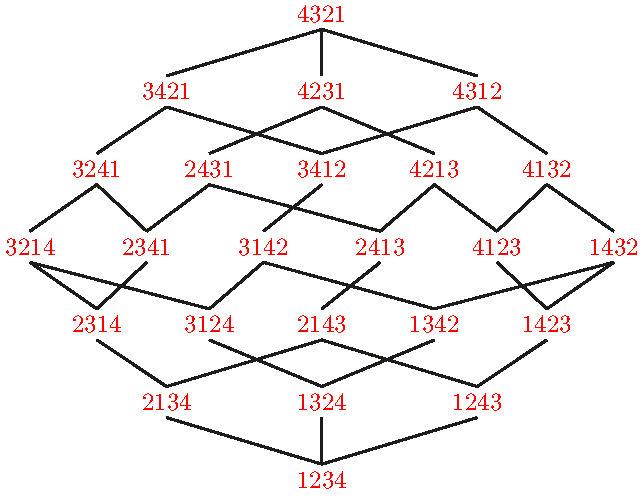
\includegraphics[scale=.55]{weakOrder}\qquad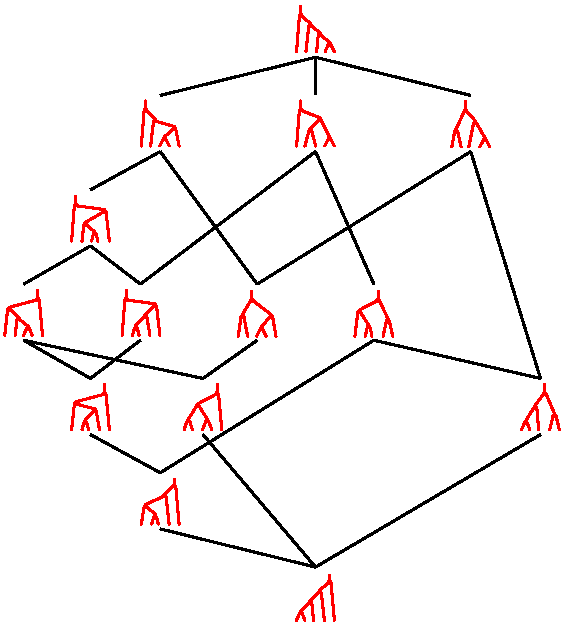
\includegraphics[scale=.45]{TamariLattice}\qquad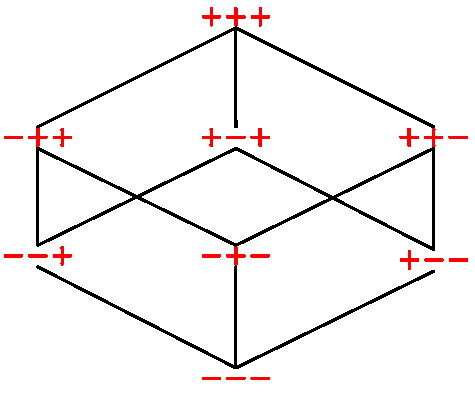
\includegraphics[scale=.7]{booleanLattice}}
	\caption{The weak order (left), the Tamari lattice (middle) and the boolean lattice (right).}
	\label{fig:classicalLattices}
\end{figure}

\begin{figure}[h]
	\centerline{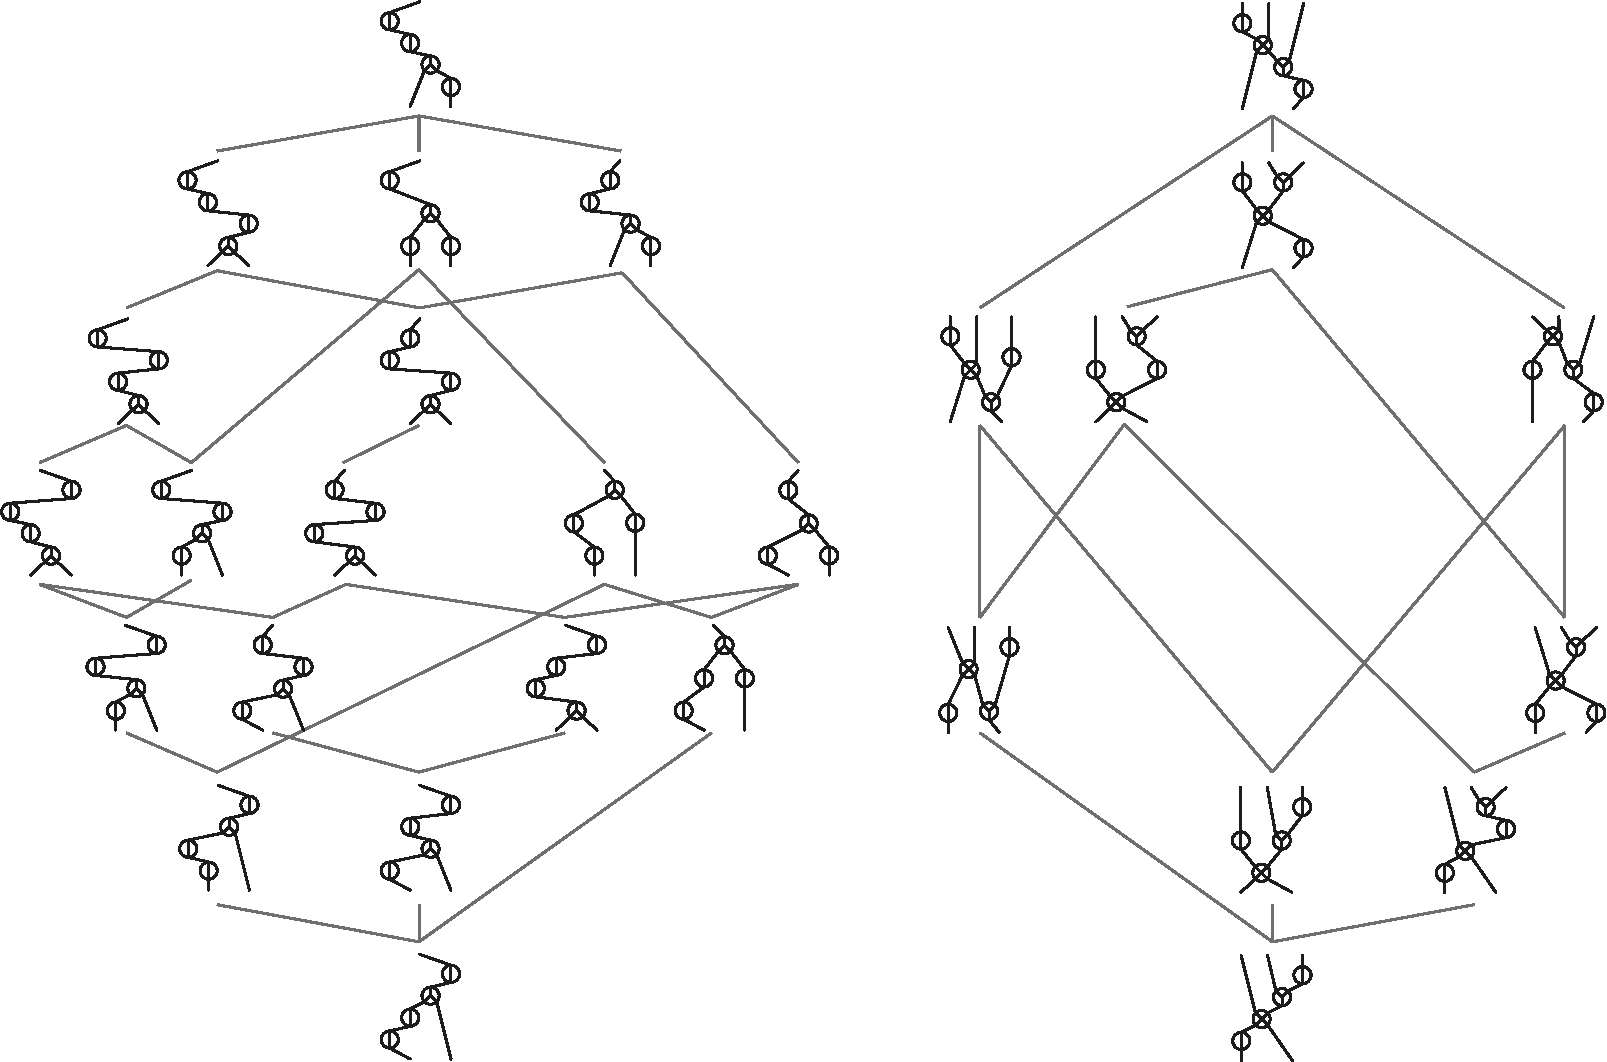
\includegraphics[scale=.5]{permutreeLattices}}
	\caption{Some permutree lattices (right).}
	\label{fig:permutreeLattices}
\end{figure}

Given a decoration~$\delta \in \Decorations$, a \defn{$\delta$-permutree}~\cite{PilaudPons-permutrees} is an oriented and labeled tree such that the node labeled~$i$ has one or two parents and one or two children depending on~$\delta_i$, and with local conditions on the labeling.
Permutrees should be consider as hybrid combinatorial objects between permutations (obtained when each node has one parent and one child), binary trees (obtained when each node has one parent and two children), and binary sequences (obtained when each node has two parents and two children).
%The $\delta$-permutrees correspond to the vertices of a polytope~$\Permutreehedron$ called \defn{permutreehedron}~\cite{PilaudPons-permutrees}.
There is also a natural rotation operation on $\delta$-permutrees, with a natural orientation, and the transitive closure of this operation defines a lattice on $\delta$-permutrees called \defn{permutree lattice} and denoted~$\cL(\delta)$.
See Fig.~\ref{fig:permutreeLattices}.
For example, the weak order on permutations is the permutree lattice~$\cL(\noneCirc^n)$, the Tamari lattice is the permutree lattice~$\cL(\downCirc^n)$, and the boolean lattice is the permutree lattice~$\cL(\upDownCirc^n)$.
The permutree lattice is always a lattice quotient of the weak order on permutations.

The objective of the internship is to develop bracket vectors of permutrees, in order to give a direct proof the increasing rotation graphs on permutrees are Hasse diagrams of lattices, without the technology of lattice quotients.

\paragraph{Scientific environment.}

The internship will take place in the GALAC team of LRI and will be cosupervised by Viviane Pons (LRI, Univ.~Orsay) and Vincent Pilaud (LIX, \'Ecole Polytechnique). The intern will benefit in particular from the weekly combinatorics seminar of the Plateau de Saclay.

%La th�se aura lieu au sein de l'�quipe Combi du LIX, et sera encadr�e par Vincent Pilaud. L'�tudiant profitera en particulier du GT Combi du Plateau de Saclay, qui permettra le contact avec les autres chercheurs en combinatoire �num�rative, alg�brique et g�om�trique du plateau de Saclay (�quipe GALaC du LRI et Combi du LIX). Les d�placements du th�sard seront soutenus par l'ANR SC$^3$\!A.

%\vspace*{-.3cm}
\bibliographystyle{alpha}
\small
\renewcommand{\refname}{\normalsize Bibliographie}
\bibliography{projetStage}
\normalsize

\end{document}